\documentclass[twoside]{book}

% Packages required by doxygen
\usepackage{fixltx2e}
\usepackage{calc}
\usepackage{doxygen}
\usepackage[export]{adjustbox} % also loads graphicx
\usepackage{graphicx}
\usepackage[utf8]{inputenc}
\usepackage{makeidx}
\usepackage{multicol}
\usepackage{multirow}
\PassOptionsToPackage{warn}{textcomp}
\usepackage{textcomp}
\usepackage[nointegrals]{wasysym}
\usepackage[table]{xcolor}

% Font selection
\usepackage[T1]{fontenc}
\usepackage[scaled=.90]{helvet}
\usepackage{courier}
\usepackage{amssymb}
\usepackage{sectsty}
\renewcommand{\familydefault}{\sfdefault}
\allsectionsfont{%
  \fontseries{bc}\selectfont%
  \color{darkgray}%
}
\renewcommand{\DoxyLabelFont}{%
  \fontseries{bc}\selectfont%
  \color{darkgray}%
}
\newcommand{\+}{\discretionary{\mbox{\scriptsize$\hookleftarrow$}}{}{}}

% Page & text layout
\usepackage{geometry}
\geometry{%
  a4paper,%
  top=2.5cm,%
  bottom=2.5cm,%
  left=2.5cm,%
  right=2.5cm%
}
\tolerance=750
\hfuzz=15pt
\hbadness=750
\setlength{\emergencystretch}{15pt}
\setlength{\parindent}{0cm}
\setlength{\parskip}{3ex plus 2ex minus 2ex}
\makeatletter
\renewcommand{\paragraph}{%
  \@startsection{paragraph}{4}{0ex}{-1.0ex}{1.0ex}{%
    \normalfont\normalsize\bfseries\SS@parafont%
  }%
}
\renewcommand{\subparagraph}{%
  \@startsection{subparagraph}{5}{0ex}{-1.0ex}{1.0ex}{%
    \normalfont\normalsize\bfseries\SS@subparafont%
  }%
}
\makeatother

% Headers & footers
\usepackage{fancyhdr}
\pagestyle{fancyplain}
\fancyhead[LE]{\fancyplain{}{\bfseries\thepage}}
\fancyhead[CE]{\fancyplain{}{}}
\fancyhead[RE]{\fancyplain{}{\bfseries\leftmark}}
\fancyhead[LO]{\fancyplain{}{\bfseries\rightmark}}
\fancyhead[CO]{\fancyplain{}{}}
\fancyhead[RO]{\fancyplain{}{\bfseries\thepage}}
\fancyfoot[LE]{\fancyplain{}{}}
\fancyfoot[CE]{\fancyplain{}{}}
\fancyfoot[RE]{\fancyplain{}{\bfseries\scriptsize Generated by Doxygen }}
\fancyfoot[LO]{\fancyplain{}{\bfseries\scriptsize Generated by Doxygen }}
\fancyfoot[CO]{\fancyplain{}{}}
\fancyfoot[RO]{\fancyplain{}{}}
\renewcommand{\footrulewidth}{0.4pt}
\renewcommand{\chaptermark}[1]{%
  \markboth{#1}{}%
}
\renewcommand{\sectionmark}[1]{%
  \markright{\thesection\ #1}%
}

% Indices & bibliography
\usepackage{natbib}
\usepackage[titles]{tocloft}
\setcounter{tocdepth}{3}
\setcounter{secnumdepth}{5}
\makeindex

% Hyperlinks (required, but should be loaded last)
\usepackage{ifpdf}
\ifpdf
  \usepackage[pdftex,pagebackref=true]{hyperref}
\else
  \usepackage[ps2pdf,pagebackref=true]{hyperref}
\fi
\hypersetup{%
  colorlinks=true,%
  linkcolor=blue,%
  citecolor=blue,%
  unicode%
}

% Custom commands
\newcommand{\clearemptydoublepage}{%
  \newpage{\pagestyle{empty}\cleardoublepage}%
}

\usepackage{caption}
\captionsetup{labelsep=space,justification=centering,font={bf},singlelinecheck=off,skip=4pt,position=top}

%===== C O N T E N T S =====

\begin{document}

% Titlepage & ToC
\hypersetup{pageanchor=false,
             bookmarksnumbered=true,
             pdfencoding=unicode
            }
\pagenumbering{alph}
\begin{titlepage}
\vspace*{7cm}
\begin{center}%
{\Large L\+P\+DM Nanogrid Simulation }\\
\vspace*{1cm}
{\large Generated by Doxygen 1.8.13}\\
\end{center}
\end{titlepage}
\clearemptydoublepage
\pagenumbering{roman}
\tableofcontents
\clearemptydoublepage
\pagenumbering{arabic}
\hypersetup{pageanchor=true}

%--- Begin generated contents ---
\chapter{Namespace Index}
\section{Packages}
Here are the packages with brief descriptions (if available)\+:\begin{DoxyCompactList}
\item\contentsline{section}{\hyperlink{namespace_device}{Device} }{\pageref{namespace_device}}{}
\item\contentsline{section}{\hyperlink{namespace_event}{Event} }{\pageref{namespace_event}}{}
\item\contentsline{section}{\hyperlink{namespace_priority__queue}{Priority\+\_\+queue} }{\pageref{namespace_priority__queue}}{}
\item\contentsline{section}{\hyperlink{namespace_supervisor}{Supervisor} }{\pageref{namespace_supervisor}}{}
\end{DoxyCompactList}

\chapter{Hierarchical Index}
\section{Class Hierarchy}
This inheritance list is sorted roughly, but not completely, alphabetically\+:\begin{DoxyCompactList}
\item Formatter\begin{DoxyCompactList}
\item \contentsline{section}{Build.\+Simulation\+\_\+\+Operation.\+logger.\+Simulation\+Logger.\+Formatter\+With\+Header}{\pageref{class_build_1_1_simulation___operation_1_1logger_1_1_simulation_logger_1_1_formatter_with_header}}{}
\end{DoxyCompactList}
\item metaclass\begin{DoxyCompactList}
\item \contentsline{section}{Build.\+Objects.\+battery.\+Battery\+Price\+Logic}{\pageref{class_build_1_1_objects_1_1battery_1_1_battery_price_logic}}{}
\begin{DoxyCompactList}
\item \contentsline{section}{Build.\+Objects.\+battery.\+Battery\+Price\+LogicA}{\pageref{class_build_1_1_objects_1_1battery_1_1_battery_price_logic_a}}{}
\item \contentsline{section}{Build.\+Objects.\+battery.\+Battery\+Price\+LogicB}{\pageref{class_build_1_1_objects_1_1battery_1_1_battery_price_logic_b}}{}
\end{DoxyCompactList}
\item \contentsline{section}{Build.\+Objects.\+device.\+Device}{\pageref{class_build_1_1_objects_1_1device_1_1_device}}{}
\begin{DoxyCompactList}
\item \contentsline{section}{Build.\+Objects.\+eud.\+Eud}{\pageref{class_build_1_1_objects_1_1eud_1_1_eud}}{}
\begin{DoxyCompactList}
\item \contentsline{section}{Build.\+Objects.\+air\+\_\+conditioner.\+Air\+Conditioner\+Simple}{\pageref{class_build_1_1_objects_1_1air__conditioner_1_1_air_conditioner_simple}}{}
\item \contentsline{section}{Build.\+Objects.\+fixed\+\_\+consumption.\+Fixed\+Consumption}{\pageref{class_build_1_1_objects_1_1fixed__consumption_1_1_fixed_consumption}}{}
\item \contentsline{section}{Build.\+Objects.\+light.\+Light}{\pageref{class_build_1_1_objects_1_1light_1_1_light}}{}
\end{DoxyCompactList}
\item \contentsline{section}{Build.\+Objects.\+grid\+\_\+controller.\+Grid\+Controller}{\pageref{class_build_1_1_objects_1_1grid__controller_1_1_grid_controller}}{}
\item \contentsline{section}{Build.\+Objects.\+grid\+\_\+equipment.\+Grid\+Equipment}{\pageref{class_build_1_1_objects_1_1grid__equipment_1_1_grid_equipment}}{}
\item \contentsline{section}{Build.\+Objects.\+pv.\+PV}{\pageref{class_build_1_1_objects_1_1pv_1_1_p_v}}{}
\item \contentsline{section}{Build.\+Objects.\+utility\+\_\+meter.\+Utility\+Meter}{\pageref{class_build_1_1_objects_1_1utility__meter_1_1_utility_meter}}{}
\end{DoxyCompactList}
\item \contentsline{section}{Build.\+Objects.\+grid\+\_\+controller.\+Grid\+Controller\+Price\+Logic}{\pageref{class_build_1_1_objects_1_1grid__controller_1_1_grid_controller_price_logic}}{}
\begin{DoxyCompactList}
\item \contentsline{section}{Build.\+Objects.\+grid\+\_\+controller.\+G\+C\+Marginal\+Price\+Logic}{\pageref{class_build_1_1_objects_1_1grid__controller_1_1_g_c_marginal_price_logic}}{}
\item \contentsline{section}{Build.\+Objects.\+grid\+\_\+controller.\+G\+C\+Marginal\+Price\+LogicB}{\pageref{class_build_1_1_objects_1_1grid__controller_1_1_g_c_marginal_price_logic_b}}{}
\item \contentsline{section}{Build.\+Objects.\+grid\+\_\+controller.\+G\+C\+Weighted\+Average\+Price\+Logic}{\pageref{class_build_1_1_objects_1_1grid__controller_1_1_g_c_weighted_average_price_logic}}{}
\end{DoxyCompactList}
\item \contentsline{section}{Build.\+Objects.\+grid\+\_\+equipment.\+Grid\+Equipment}{\pageref{class_build_1_1_objects_1_1grid__equipment_1_1_grid_equipment}}{}
\end{DoxyCompactList}
\item object\begin{DoxyCompactList}
\item \contentsline{section}{Build.\+Objects.\+battery.\+Battery}{\pageref{class_build_1_1_objects_1_1battery_1_1_battery}}{}
\item \contentsline{section}{Build.\+Simulation\+\_\+\+Operation.\+event.\+Event}{\pageref{class_build_1_1_simulation___operation_1_1event_1_1_event}}{}
\item \contentsline{section}{Build.\+Simulation\+\_\+\+Operation.\+message.\+Message}{\pageref{class_build_1_1_simulation___operation_1_1message_1_1_message}}{}
\end{DoxyCompactList}
\item \contentsline{section}{Build.\+Simulation\+\_\+\+Operation.\+queue.\+Priority\+Queue}{\pageref{class_build_1_1_simulation___operation_1_1queue_1_1_priority_queue}}{}
\item \contentsline{section}{Build.\+Simulation\+\_\+\+Operation.\+logger.\+Simulation\+Logger}{\pageref{class_build_1_1_simulation___operation_1_1logger_1_1_simulation_logger}}{}
\item \contentsline{section}{Build.\+Simulation\+\_\+\+Operation.\+simulation.\+Simulation\+Setup}{\pageref{class_build_1_1_simulation___operation_1_1simulation_1_1_simulation_setup}}{}
\item \contentsline{section}{Build.\+Simulation\+\_\+\+Operation.\+supervisor.\+Supervisor}{\pageref{class_build_1_1_simulation___operation_1_1supervisor_1_1_supervisor}}{}
\item \contentsline{section}{Build.\+Objects.\+wire.\+Wire}{\pageref{class_build_1_1_objects_1_1wire_1_1_wire}}{}
\item A\+B\+C\+Meta\begin{DoxyCompactList}
\item \contentsline{section}{Build.\+Objects.\+battery.\+Battery\+Price\+Logic}{\pageref{class_build_1_1_objects_1_1battery_1_1_battery_price_logic}}{}
\item \contentsline{section}{Build.\+Objects.\+device.\+Device}{\pageref{class_build_1_1_objects_1_1device_1_1_device}}{}
\item \contentsline{section}{Build.\+Objects.\+grid\+\_\+controller.\+Grid\+Controller\+Price\+Logic}{\pageref{class_build_1_1_objects_1_1grid__controller_1_1_grid_controller_price_logic}}{}
\item \contentsline{section}{Build.\+Objects.\+grid\+\_\+equipment.\+Grid\+Equipment}{\pageref{class_build_1_1_objects_1_1grid__equipment_1_1_grid_equipment}}{}
\end{DoxyCompactList}
\item Enum\begin{DoxyCompactList}
\item \contentsline{section}{Build.\+Objects.\+battery.\+Battery.\+Battery\+Charging\+Preference}{\pageref{class_build_1_1_objects_1_1battery_1_1_battery_1_1_battery_charging_preference}}{}
\item \contentsline{section}{Build.\+Simulation\+\_\+\+Operation.\+message.\+Message\+Type}{\pageref{class_build_1_1_simulation___operation_1_1message_1_1_message_type}}{}
\end{DoxyCompactList}
\end{DoxyCompactList}

\chapter{Class Index}
\section{Class List}
Here are the classes, structs, unions and interfaces with brief descriptions\+:\begin{DoxyCompactList}
\item\contentsline{section}{\hyperlink{class_device_1_1_device}{Device.\+Device} }{\pageref{class_device_1_1_device}}{}
\item\contentsline{section}{\hyperlink{class_e_u_d_1_1_eud}{E\+U\+D.\+Eud} }{\pageref{class_e_u_d_1_1_eud}}{}
\item\contentsline{section}{\hyperlink{class_event_1_1_event}{Event.\+Event} }{\pageref{class_event_1_1_event}}{}
\item\contentsline{section}{\hyperlink{class_message_1_1_message}{Message.\+Message} \\*A class to represent messages passed between devices }{\pageref{class_message_1_1_message}}{}
\item\contentsline{section}{\hyperlink{class_message_1_1_message_type}{Message.\+Message\+Type} \\*Messages can be of three types\+: Register, power, and price }{\pageref{class_message_1_1_message_type}}{}
\item\contentsline{section}{\hyperlink{class_priority__queue_1_1_priority_queue}{Priority\+\_\+queue.\+Priority\+Queue} }{\pageref{class_priority__queue_1_1_priority_queue}}{}
\item\contentsline{section}{\hyperlink{class_supervisor_1_1_supervisor}{Supervisor.\+Supervisor} }{\pageref{class_supervisor_1_1_supervisor}}{}
\end{DoxyCompactList}

\chapter{Namespace Documentation}
\hypertarget{namespace_device}{}\section{Device Namespace Reference}
\label{namespace_device}\index{Device@{Device}}
\subsection*{Classes}
\begin{DoxyCompactItemize}
\item 
class \hyperlink{class_device_1_1_device}{Device}
\end{DoxyCompactItemize}


\subsection{Detailed Description}
\begin{DoxyVerb}A device maintains a priority queue of functions prioritized by time.
The queue is a heap sorted by by time signature, with time in milliseconds from the current time for the event to be processed.
The\end{DoxyVerb}
 
\hypertarget{namespace_event}{}\section{Event Namespace Reference}
\label{namespace_event}\index{Event@{Event}}
\subsection*{Classes}
\begin{DoxyCompactItemize}
\item 
class \hyperlink{class_event_1_1_event}{Event}
\end{DoxyCompactItemize}


\subsection{Detailed Description}
\begin{DoxyVerb}An event is modelled as a function call with a specified series of arguments.
Thus, it is some action that will be performed during the simulation.
The time of an event's execution is stored in the queue of devices\end{DoxyVerb}
 
\hypertarget{namespace_priority__queue}{}\section{Priority\+\_\+queue Namespace Reference}
\label{namespace_priority__queue}\index{Priority\+\_\+queue@{Priority\+\_\+queue}}
\subsection*{Classes}
\begin{DoxyCompactItemize}
\item 
class \hyperlink{class_priority__queue_1_1_priority_queue}{Priority\+Queue}
\end{DoxyCompactItemize}


\subsection{Detailed Description}
\begin{DoxyVerb}A priority queue implementing a queue of items sorted by priority.
Adapted from https://docs.python.org/2/library/heapq.html.
\end{DoxyVerb}
 
\hypertarget{namespace_supervisor}{}\section{Supervisor Namespace Reference}
\label{namespace_supervisor}\index{Supervisor@{Supervisor}}
\subsection*{Classes}
\begin{DoxyCompactItemize}
\item 
class \hyperlink{class_supervisor_1_1_supervisor}{Supervisor}
\end{DoxyCompactItemize}


\subsection{Detailed Description}
\begin{DoxyVerb}\end{DoxyVerb}
 
\chapter{Class Documentation}
\hypertarget{class_device_1_1_device}{}\section{Device.\+Device Class Reference}
\label{class_device_1_1_device}\index{Device.\+Device@{Device.\+Device}}
\subsection*{Public Member Functions}
\begin{DoxyCompactItemize}
\item 
\mbox{\Hypertarget{class_device_1_1_device_a9466bb46f9466112557bd694db6ee0b9}\label{class_device_1_1_device_a9466bb46f9466112557bd694db6ee0b9}} 
def {\bfseries \+\_\+\+\_\+init\+\_\+\+\_\+} (self, device\+\_\+id, supervisor)
\item 
def \hyperlink{class_device_1_1_device_a48c0cd986e11f67d2373871ade40992e}{add\+\_\+event} (self, event, time\+\_\+stamp)
\begin{DoxyCompactList}\small\item\em Adds an event to the device\textquotesingle{}s event queue and reports that event to the supervisor. \end{DoxyCompactList}\item 
def \hyperlink{class_device_1_1_device_a3aef2a6e416795690e9b697b3fcf4d76}{get\+\_\+id} (self)
\begin{DoxyCompactList}\small\item\em Getter for the \hyperlink{class_device_1_1_device}{Device}\textquotesingle{}s ID We maintain ID as a protected field to avoid external modifications during messaging. \end{DoxyCompactList}\item 
def \hyperlink{class_device_1_1_device_afd1b29eb311904ffa8565fd2d2079967}{process\+\_\+events} (self, run\+\_\+time)
\begin{DoxyCompactList}\small\item\em Process all events in the device\textquotesingle{}s queue with a given time\+\_\+stamp. \end{DoxyCompactList}\item 
def \hyperlink{class_device_1_1_device_abb9e113d3aba9118bbd205198e656b7a}{report\+\_\+next\+\_\+event\+\_\+time} (self)
\begin{DoxyCompactList}\small\item\em Report the time of the next earliest event in the device\textquotesingle{}s event queue. \end{DoxyCompactList}\item 
\mbox{\Hypertarget{class_device_1_1_device_ab19f8e64e8a68ecd5316db800db01d46}\label{class_device_1_1_device_ab19f8e64e8a68ecd5316db800db01d46}} 
def \hyperlink{class_device_1_1_device_ab19f8e64e8a68ecd5316db800db01d46}{receive\+\_\+message} (self, message)
\begin{DoxyCompactList}\small\item\em Receiving a message is modelled as putting an event with the message 1 time step after the function call. \end{DoxyCompactList}\item 
def \hyperlink{class_device_1_1_device_a1d4ccc0c3994e92d6c0cc22b0484801e}{read\+\_\+message} (self, message)
\item 
def \hyperlink{class_device_1_1_device_adc0a8678e0a0889ab254061e378be6fe}{register\+\_\+device} (self, device, value)
\begin{DoxyCompactList}\small\item\em Registers or unregisters a given device from the device\textquotesingle{}s connected device list. \end{DoxyCompactList}\item 
def \hyperlink{class_device_1_1_device_ac8cec0e5eee2635bc306f765e60c2f9c}{on\+\_\+power\+\_\+change} (self, new\+\_\+power)
\begin{DoxyCompactList}\small\item\em Method to be called when the device receives a power message, indicating power flows have changed between two devices (either receiving or providing). \end{DoxyCompactList}\item 
def \hyperlink{class_device_1_1_device_a2e57c6f8bccdf4644b7332284651e120}{on\+\_\+price\+\_\+change} (self, new\+\_\+price)
\begin{DoxyCompactList}\small\item\em Method to be called when device receives a price message. \end{DoxyCompactList}\item 
def \hyperlink{class_device_1_1_device_a5261b7396dd1581d649d629fccf3029c}{on\+\_\+request} (self)
\begin{DoxyCompactList}\small\item\em Method to be called when device receives a request message, indicating a device is requesting to either provide or receive the requested quantity of power. \end{DoxyCompactList}\item 
\mbox{\Hypertarget{class_device_1_1_device_a329080b5f36e73fe6b37096f408b07b7}\label{class_device_1_1_device_a329080b5f36e73fe6b37096f408b07b7}} 
def {\bfseries on\+\_\+allocate} (self)
\end{DoxyCompactItemize}


\subsection{Member Function Documentation}
\mbox{\Hypertarget{class_device_1_1_device_a48c0cd986e11f67d2373871ade40992e}\label{class_device_1_1_device_a48c0cd986e11f67d2373871ade40992e}} 
\index{Device\+::\+Device@{Device\+::\+Device}!add\+\_\+event@{add\+\_\+event}}
\index{add\+\_\+event@{add\+\_\+event}!Device\+::\+Device@{Device\+::\+Device}}
\subsubsection{\texorpdfstring{add\+\_\+event()}{add\_event()}}
{\footnotesize\ttfamily def Device.\+Device.\+add\+\_\+event (\begin{DoxyParamCaption}\item[{}]{self,  }\item[{}]{event,  }\item[{}]{time\+\_\+stamp }\end{DoxyParamCaption})}



Adds an event to the device\textquotesingle{}s event queue and reports that event to the supervisor. 


\begin{DoxyParams}{Parameters}
{\em event} & the event to add to the event queue \\
\hline
{\em time\+\_\+stamp} & the time to associate with the event in the queue \\
\hline
\end{DoxyParams}
\mbox{\Hypertarget{class_device_1_1_device_a3aef2a6e416795690e9b697b3fcf4d76}\label{class_device_1_1_device_a3aef2a6e416795690e9b697b3fcf4d76}} 
\index{Device\+::\+Device@{Device\+::\+Device}!get\+\_\+id@{get\+\_\+id}}
\index{get\+\_\+id@{get\+\_\+id}!Device\+::\+Device@{Device\+::\+Device}}
\subsubsection{\texorpdfstring{get\+\_\+id()}{get\_id()}}
{\footnotesize\ttfamily def Device.\+Device.\+get\+\_\+id (\begin{DoxyParamCaption}\item[{}]{self }\end{DoxyParamCaption})}



Getter for the \hyperlink{class_device_1_1_device}{Device}\textquotesingle{}s ID We maintain ID as a protected field to avoid external modifications during messaging. 

\begin{DoxyReturn}{Returns}
the device\textquotesingle{}s ID 
\end{DoxyReturn}
\mbox{\Hypertarget{class_device_1_1_device_ac8cec0e5eee2635bc306f765e60c2f9c}\label{class_device_1_1_device_ac8cec0e5eee2635bc306f765e60c2f9c}} 
\index{Device\+::\+Device@{Device\+::\+Device}!on\+\_\+power\+\_\+change@{on\+\_\+power\+\_\+change}}
\index{on\+\_\+power\+\_\+change@{on\+\_\+power\+\_\+change}!Device\+::\+Device@{Device\+::\+Device}}
\subsubsection{\texorpdfstring{on\+\_\+power\+\_\+change()}{on\_power\_change()}}
{\footnotesize\ttfamily def Device.\+Device.\+on\+\_\+power\+\_\+change (\begin{DoxyParamCaption}\item[{}]{self,  }\item[{}]{new\+\_\+power }\end{DoxyParamCaption})}



Method to be called when the device receives a power message, indicating power flows have changed between two devices (either receiving or providing). 


\begin{DoxyParams}{Parameters}
{\em new\+\_\+power} & the value of power flow, negative if receiving, positive if providing. \\
\hline
\end{DoxyParams}
\mbox{\Hypertarget{class_device_1_1_device_a2e57c6f8bccdf4644b7332284651e120}\label{class_device_1_1_device_a2e57c6f8bccdf4644b7332284651e120}} 
\index{Device\+::\+Device@{Device\+::\+Device}!on\+\_\+price\+\_\+change@{on\+\_\+price\+\_\+change}}
\index{on\+\_\+price\+\_\+change@{on\+\_\+price\+\_\+change}!Device\+::\+Device@{Device\+::\+Device}}
\subsubsection{\texorpdfstring{on\+\_\+price\+\_\+change()}{on\_price\_change()}}
{\footnotesize\ttfamily def Device.\+Device.\+on\+\_\+price\+\_\+change (\begin{DoxyParamCaption}\item[{}]{self,  }\item[{}]{new\+\_\+price }\end{DoxyParamCaption})}



Method to be called when device receives a price message. 


\begin{DoxyParams}{Parameters}
{\em new\+\_\+price} & the new price value \\
\hline
\end{DoxyParams}
\mbox{\Hypertarget{class_device_1_1_device_a5261b7396dd1581d649d629fccf3029c}\label{class_device_1_1_device_a5261b7396dd1581d649d629fccf3029c}} 
\index{Device\+::\+Device@{Device\+::\+Device}!on\+\_\+request@{on\+\_\+request}}
\index{on\+\_\+request@{on\+\_\+request}!Device\+::\+Device@{Device\+::\+Device}}
\subsubsection{\texorpdfstring{on\+\_\+request()}{on\_request()}}
{\footnotesize\ttfamily def Device.\+Device.\+on\+\_\+request (\begin{DoxyParamCaption}\item[{}]{self }\end{DoxyParamCaption})}



Method to be called when device receives a request message, indicating a device is requesting to either provide or receive the requested quantity of power. 


\begin{DoxyParams}{Parameters}
{\em new\+\_\+price} & the new price value \\
\hline
\end{DoxyParams}
\mbox{\Hypertarget{class_device_1_1_device_afd1b29eb311904ffa8565fd2d2079967}\label{class_device_1_1_device_afd1b29eb311904ffa8565fd2d2079967}} 
\index{Device\+::\+Device@{Device\+::\+Device}!process\+\_\+events@{process\+\_\+events}}
\index{process\+\_\+events@{process\+\_\+events}!Device\+::\+Device@{Device\+::\+Device}}
\subsubsection{\texorpdfstring{process\+\_\+events()}{process\_events()}}
{\footnotesize\ttfamily def Device.\+Device.\+process\+\_\+events (\begin{DoxyParamCaption}\item[{}]{self,  }\item[{}]{run\+\_\+time }\end{DoxyParamCaption})}



Process all events in the device\textquotesingle{}s queue with a given time\+\_\+stamp. 

This function should be called after advance\+\_\+time has been called by the supervisor. \mbox{\Hypertarget{class_device_1_1_device_a1d4ccc0c3994e92d6c0cc22b0484801e}\label{class_device_1_1_device_a1d4ccc0c3994e92d6c0cc22b0484801e}} 
\index{Device\+::\+Device@{Device\+::\+Device}!read\+\_\+message@{read\+\_\+message}}
\index{read\+\_\+message@{read\+\_\+message}!Device\+::\+Device@{Device\+::\+Device}}
\subsubsection{\texorpdfstring{read\+\_\+message()}{read\_message()}}
{\footnotesize\ttfamily def Device.\+Device.\+read\+\_\+message (\begin{DoxyParamCaption}\item[{}]{self,  }\item[{}]{message }\end{DoxyParamCaption})}


\begin{DoxyParams}{Parameters}
{\em message} & a message to be read (must be a message object) \\
\hline
\end{DoxyParams}
\mbox{\Hypertarget{class_device_1_1_device_adc0a8678e0a0889ab254061e378be6fe}\label{class_device_1_1_device_adc0a8678e0a0889ab254061e378be6fe}} 
\index{Device\+::\+Device@{Device\+::\+Device}!register\+\_\+device@{register\+\_\+device}}
\index{register\+\_\+device@{register\+\_\+device}!Device\+::\+Device@{Device\+::\+Device}}
\subsubsection{\texorpdfstring{register\+\_\+device()}{register\_device()}}
{\footnotesize\ttfamily def Device.\+Device.\+register\+\_\+device (\begin{DoxyParamCaption}\item[{}]{self,  }\item[{}]{device,  }\item[{}]{value }\end{DoxyParamCaption})}



Registers or unregisters a given device from the device\textquotesingle{}s connected device list. 


\begin{DoxyParams}{Parameters}
{\em device} & the device to register or unregister from connected devices \\
\hline
{\em value} & positive to register, 0 or negative to unregister \\
\hline
\end{DoxyParams}
\mbox{\Hypertarget{class_device_1_1_device_abb9e113d3aba9118bbd205198e656b7a}\label{class_device_1_1_device_abb9e113d3aba9118bbd205198e656b7a}} 
\index{Device\+::\+Device@{Device\+::\+Device}!report\+\_\+next\+\_\+event\+\_\+time@{report\+\_\+next\+\_\+event\+\_\+time}}
\index{report\+\_\+next\+\_\+event\+\_\+time@{report\+\_\+next\+\_\+event\+\_\+time}!Device\+::\+Device@{Device\+::\+Device}}
\subsubsection{\texorpdfstring{report\+\_\+next\+\_\+event\+\_\+time()}{report\_next\_event\_time()}}
{\footnotesize\ttfamily def Device.\+Device.\+report\+\_\+next\+\_\+event\+\_\+time (\begin{DoxyParamCaption}\item[{}]{self }\end{DoxyParamCaption})}



Report the time of the next earliest event in the device\textquotesingle{}s event queue. 

\begin{DoxyReturn}{Returns}
a tuple of device\textquotesingle{}s ID and the time of its next event 
\end{DoxyReturn}


The documentation for this class was generated from the following file\+:\begin{DoxyCompactItemize}
\item 
Build/Device.\+py\end{DoxyCompactItemize}

\hypertarget{class_e_u_d_1_1_eud}{}\section{E\+U\+D.\+Eud Class Reference}
\label{class_e_u_d_1_1_eud}\index{E\+U\+D.\+Eud@{E\+U\+D.\+Eud}}
Inheritance diagram for E\+U\+D.\+Eud\+:\begin{figure}[H]
\begin{center}
\leavevmode
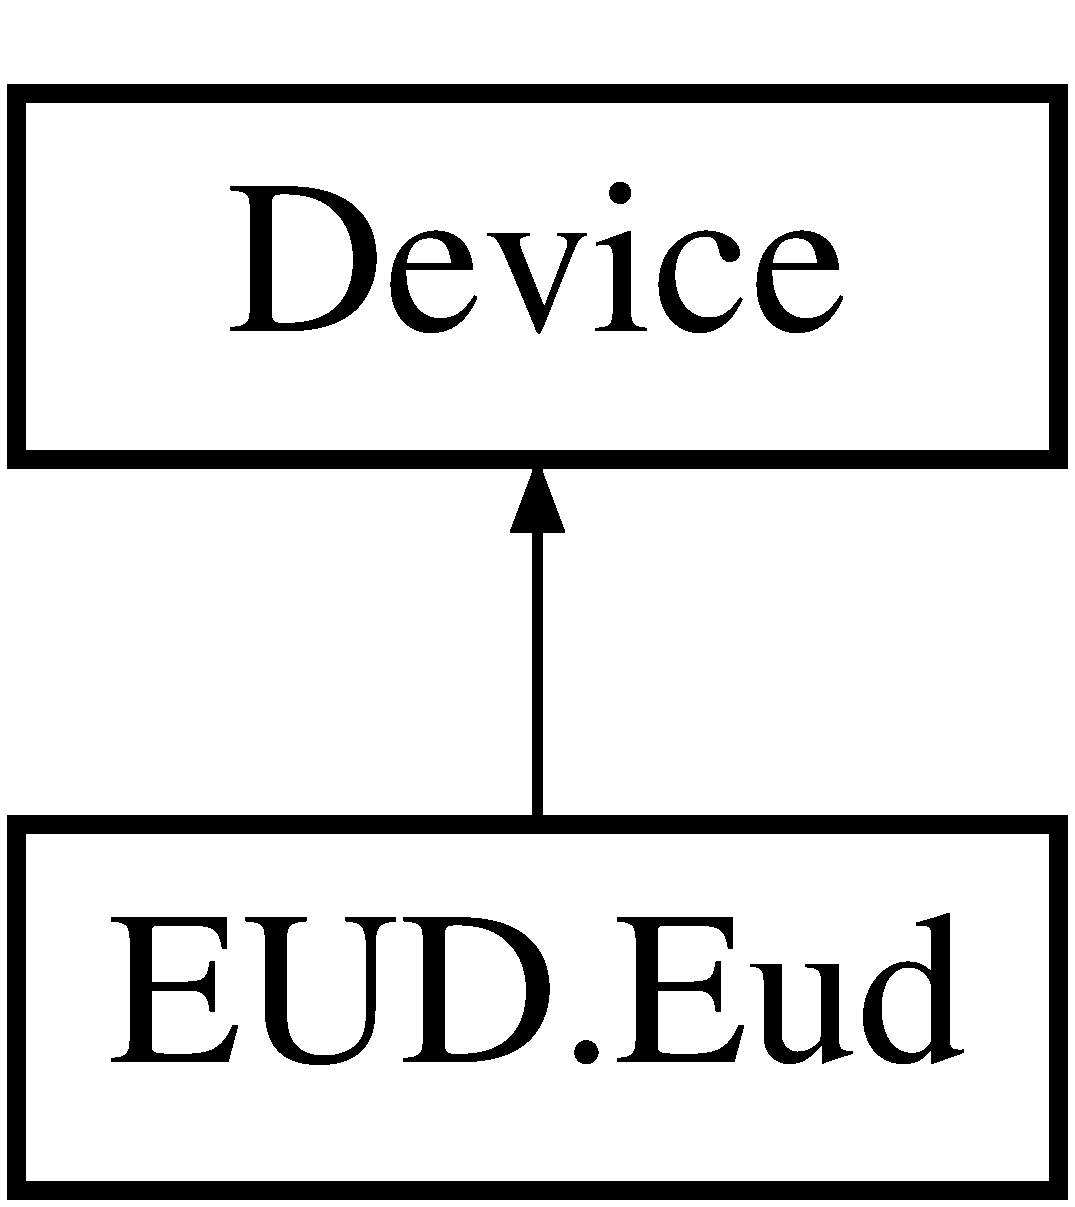
\includegraphics[height=2.000000cm]{class_e_u_d_1_1_eud}
\end{center}
\end{figure}
\subsection*{Public Member Functions}
\begin{DoxyCompactItemize}
\item 
\mbox{\Hypertarget{class_e_u_d_1_1_eud_ae051ec0c4270509aa988b5ae9a989055}\label{class_e_u_d_1_1_eud_ae051ec0c4270509aa988b5ae9a989055}} 
def {\bfseries \+\_\+\+\_\+init\+\_\+\+\_\+} (self, device\+\_\+id, supervisor)
\item 
\mbox{\Hypertarget{class_e_u_d_1_1_eud_a2cb2f8d68e0dcff8da5078ca0d954af4}\label{class_e_u_d_1_1_eud_a2cb2f8d68e0dcff8da5078ca0d954af4}} 
def {\bfseries on\+\_\+power\+\_\+change} (self, source\+\_\+device\+\_\+id, target\+\_\+device\+\_\+id, time, new\+\_\+power)
\item 
\mbox{\Hypertarget{class_e_u_d_1_1_eud_a62e7b3e5e8395a2d70be4d8967735aa4}\label{class_e_u_d_1_1_eud_a62e7b3e5e8395a2d70be4d8967735aa4}} 
def {\bfseries on\+\_\+capacity\+\_\+change} (self, source\+\_\+device\+\_\+id, target\+\_\+device\+\_\+id, time, value)
\item 
\mbox{\Hypertarget{class_e_u_d_1_1_eud_aaa9ef93d0c1635f310bec04a9c214b61}\label{class_e_u_d_1_1_eud_aaa9ef93d0c1635f310bec04a9c214b61}} 
def {\bfseries on\+\_\+price\+\_\+change} (self, source\+\_\+device\+\_\+id, target\+\_\+device\+\_\+id, time, new\+\_\+price)
\item 
\mbox{\Hypertarget{class_e_u_d_1_1_eud_af75ff7597f0adc361b62d790f531c213}\label{class_e_u_d_1_1_eud_af75ff7597f0adc361b62d790f531c213}} 
def {\bfseries on\+\_\+time\+\_\+change} (self, new\+\_\+time)
\item 
\mbox{\Hypertarget{class_e_u_d_1_1_eud_a206a8e7705cb533ab86a524897572f68}\label{class_e_u_d_1_1_eud_a206a8e7705cb533ab86a524897572f68}} 
def {\bfseries process\+\_\+events} (self)
\item 
\mbox{\Hypertarget{class_e_u_d_1_1_eud_a669adf7a73efad185dbee1daa6f0e5d2}\label{class_e_u_d_1_1_eud_a669adf7a73efad185dbee1daa6f0e5d2}} 
def {\bfseries set\+\_\+allocated} (self, allocate)
\item 
\mbox{\Hypertarget{class_e_u_d_1_1_eud_a8580909e552286ccb855132722a84f29}\label{class_e_u_d_1_1_eud_a8580909e552286ccb855132722a84f29}} 
def {\bfseries send\+\_\+request} (self, request)
\end{DoxyCompactItemize}
\subsection*{Public Attributes}
\begin{DoxyCompactItemize}
\item 
\mbox{\Hypertarget{class_e_u_d_1_1_eud_ac9aceff0e06b670cd661021e54b9d09f}\label{class_e_u_d_1_1_eud_ac9aceff0e06b670cd661021e54b9d09f}} 
{\bfseries allocated}
\end{DoxyCompactItemize}


The documentation for this class was generated from the following file\+:\begin{DoxyCompactItemize}
\item 
Build/E\+U\+D.\+py\end{DoxyCompactItemize}

\hypertarget{class_event_1_1_event}{}\section{Event.\+Event Class Reference}
\label{class_event_1_1_event}\index{Event.\+Event@{Event.\+Event}}
\subsection*{Public Member Functions}
\begin{DoxyCompactItemize}
\item 
def \hyperlink{class_event_1_1_event_a59dde669156fd5abc94b3800ece49b36}{\+\_\+\+\_\+init\+\_\+\+\_\+} (self, action, args)
\begin{DoxyCompactList}\small\item\em Initialize an event with a function and arguments for that function. \end{DoxyCompactList}\item 
def \hyperlink{class_event_1_1_event_a06520d9b62a64266891af59f31c5ccad}{run\+\_\+event} (self)
\begin{DoxyCompactList}\small\item\em Initialize an event with a function and arguments for that function. \end{DoxyCompactList}\end{DoxyCompactItemize}


\subsection{Constructor \& Destructor Documentation}
\mbox{\Hypertarget{class_event_1_1_event_a59dde669156fd5abc94b3800ece49b36}\label{class_event_1_1_event_a59dde669156fd5abc94b3800ece49b36}} 
\index{Event\+::\+Event@{Event\+::\+Event}!\+\_\+\+\_\+init\+\_\+\+\_\+@{\+\_\+\+\_\+init\+\_\+\+\_\+}}
\index{\+\_\+\+\_\+init\+\_\+\+\_\+@{\+\_\+\+\_\+init\+\_\+\+\_\+}!Event\+::\+Event@{Event\+::\+Event}}
\subsubsection{\texorpdfstring{\+\_\+\+\_\+init\+\_\+\+\_\+()}{\_\_init\_\_()}}
{\footnotesize\ttfamily def Event.\+Event.\+\_\+\+\_\+init\+\_\+\+\_\+ (\begin{DoxyParamCaption}\item[{}]{self,  }\item[{}]{action,  }\item[{}]{args }\end{DoxyParamCaption})}



Initialize an event with a function and arguments for that function. 


\begin{DoxyParams}{Parameters}
{\em action} & a function with {\bfseries no return type} to be run in the event \\
\hline
{\em args} & a tuple of arguments for the function \\
\hline
\end{DoxyParams}


\subsection{Member Function Documentation}
\mbox{\Hypertarget{class_event_1_1_event_a06520d9b62a64266891af59f31c5ccad}\label{class_event_1_1_event_a06520d9b62a64266891af59f31c5ccad}} 
\index{Event\+::\+Event@{Event\+::\+Event}!run\+\_\+event@{run\+\_\+event}}
\index{run\+\_\+event@{run\+\_\+event}!Event\+::\+Event@{Event\+::\+Event}}
\subsubsection{\texorpdfstring{run\+\_\+event()}{run\_event()}}
{\footnotesize\ttfamily def Event.\+Event.\+run\+\_\+event (\begin{DoxyParamCaption}\item[{}]{self }\end{DoxyParamCaption})}



Initialize an event with a function and arguments for that function. 


\begin{DoxyParams}{Parameters}
{\em action} & a function to be run in the event \\
\hline
{\em args} & a tuple of arguments for the function \\
\hline
\end{DoxyParams}


The documentation for this class was generated from the following file\+:\begin{DoxyCompactItemize}
\item 
Build/Event.\+py\end{DoxyCompactItemize}

\hypertarget{class_message_1_1_message}{}\section{Message.\+Message Class Reference}
\label{class_message_1_1_message}\index{Message.\+Message@{Message.\+Message}}


A class to represent messages passed between devices.  


\subsection*{Public Member Functions}
\begin{DoxyCompactItemize}
\item 
\mbox{\Hypertarget{class_message_1_1_message_a62fda57019b81f4ab2530c9b1cf9b363}\label{class_message_1_1_message_a62fda57019b81f4ab2530c9b1cf9b363}} 
def {\bfseries \+\_\+\+\_\+init\+\_\+\+\_\+} (self, time, sender, message\+\_\+type, value)
\end{DoxyCompactItemize}
\subsection*{Public Attributes}
\begin{DoxyCompactItemize}
\item 
\mbox{\Hypertarget{class_message_1_1_message_a5c41eff29d23d4a89f4ff32e6d2ee1f0}\label{class_message_1_1_message_a5c41eff29d23d4a89f4ff32e6d2ee1f0}} 
{\bfseries time}
\item 
\mbox{\Hypertarget{class_message_1_1_message_aac5c3be100e21c16277823abd73f1efa}\label{class_message_1_1_message_aac5c3be100e21c16277823abd73f1efa}} 
{\bfseries sender}
\item 
\mbox{\Hypertarget{class_message_1_1_message_a903b0cd428b5718873b4500635ca93fb}\label{class_message_1_1_message_a903b0cd428b5718873b4500635ca93fb}} 
{\bfseries message\+\_\+type}
\item 
\mbox{\Hypertarget{class_message_1_1_message_a1b7415657dc4705dc68e94b1417e963b}\label{class_message_1_1_message_a1b7415657dc4705dc68e94b1417e963b}} 
{\bfseries value}
\end{DoxyCompactItemize}


\subsection{Detailed Description}
A class to represent messages passed between devices. 



The documentation for this class was generated from the following file\+:\begin{DoxyCompactItemize}
\item 
Build/Message.\+py\end{DoxyCompactItemize}

\hypertarget{class_message_1_1_message_type}{}\section{Message.\+Message\+Type Class Reference}
\label{class_message_1_1_message_type}\index{Message.\+Message\+Type@{Message.\+Message\+Type}}


Messages can be of three types\+: Register, power, and price.  


Inheritance diagram for Message.\+Message\+Type\+:\begin{figure}[H]
\begin{center}
\leavevmode
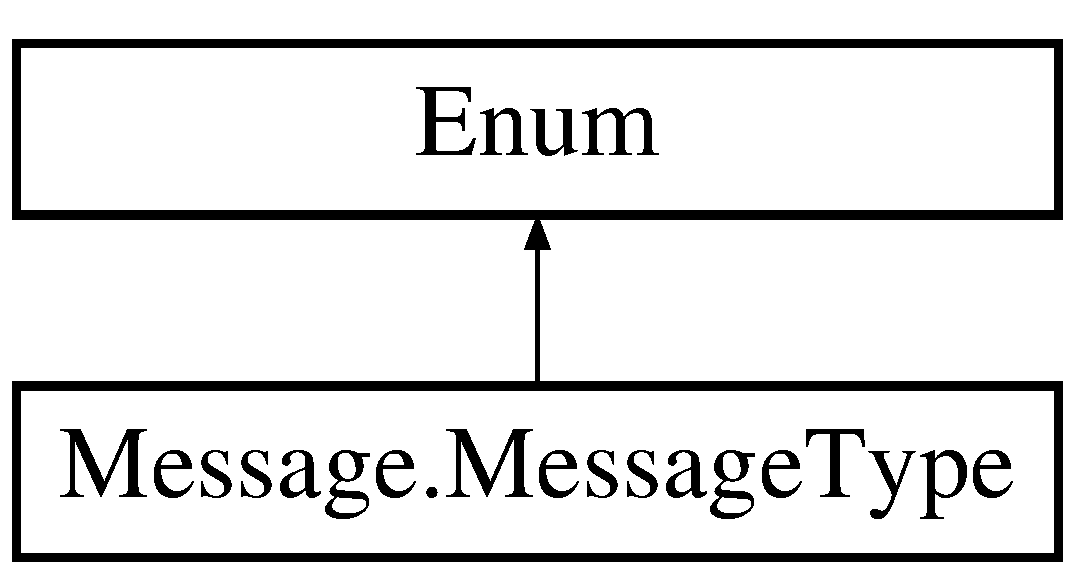
\includegraphics[height=2.000000cm]{class_message_1_1_message_type}
\end{center}
\end{figure}
\subsection*{Static Public Attributes}
\begin{DoxyCompactItemize}
\item 
\mbox{\Hypertarget{class_message_1_1_message_type_a0d0bb9f07984aa93f046573f72a84035}\label{class_message_1_1_message_type_a0d0bb9f07984aa93f046573f72a84035}} 
int {\bfseries R\+E\+G\+I\+S\+T\+ER} = 1
\item 
\mbox{\Hypertarget{class_message_1_1_message_type_ae225efff6af9ca0747fe3a132f320c75}\label{class_message_1_1_message_type_ae225efff6af9ca0747fe3a132f320c75}} 
int {\bfseries P\+O\+W\+ER} = 2
\item 
\mbox{\Hypertarget{class_message_1_1_message_type_a99b0232e6ae0f357b5b0bd524c01415c}\label{class_message_1_1_message_type_a99b0232e6ae0f357b5b0bd524c01415c}} 
int {\bfseries P\+R\+I\+CE} = 3
\item 
\mbox{\Hypertarget{class_message_1_1_message_type_a7e25f21a4f68319bbe96aa9356b1d77f}\label{class_message_1_1_message_type_a7e25f21a4f68319bbe96aa9356b1d77f}} 
int {\bfseries R\+E\+Q\+U\+E\+ST} = 4
\item 
\mbox{\Hypertarget{class_message_1_1_message_type_adf30ed0f375640a996f380adb3fc1e06}\label{class_message_1_1_message_type_adf30ed0f375640a996f380adb3fc1e06}} 
int {\bfseries A\+L\+L\+O\+C\+A\+TE} = 5
\end{DoxyCompactItemize}


\subsection{Detailed Description}
Messages can be of three types\+: Register, power, and price. 

A register message indicates that a device is seeking to register or unregister a connection with another device; a positive value with Register indicates that it would like to be registered under that device\textquotesingle{}s connected devices, while a negative value indicates that it is requesting to disconnect.

A power message indicates that a device is seeking to obtain or sell a quantity of power to/from another device. A positive value indicates that it wants to sell that amount, while a negative value indicates that it would like to purchase that amount. 

The documentation for this class was generated from the following file\+:\begin{DoxyCompactItemize}
\item 
Build/Message.\+py\end{DoxyCompactItemize}

\hypertarget{class_priority__queue_1_1_priority_queue}{}\section{Priority\+\_\+queue.\+Priority\+Queue Class Reference}
\label{class_priority__queue_1_1_priority_queue}\index{Priority\+\_\+queue.\+Priority\+Queue@{Priority\+\_\+queue.\+Priority\+Queue}}
\subsection*{Public Member Functions}
\begin{DoxyCompactItemize}
\item 
\mbox{\Hypertarget{class_priority__queue_1_1_priority_queue_aa64e91440263bad56792ef1a94ef8c60}\label{class_priority__queue_1_1_priority_queue_aa64e91440263bad56792ef1a94ef8c60}} 
def {\bfseries \+\_\+\+\_\+init\+\_\+\+\_\+} (self)
\item 
def \hyperlink{class_priority__queue_1_1_priority_queue_a4655c59199cd1a181db01b265c0bd84d}{add} (self, task, priority=0)
\item 
def \hyperlink{class_priority__queue_1_1_priority_queue_a311e92d0a6c8a26393d9122b159d6b17}{remove} (self, task)
\item 
def \hyperlink{class_priority__queue_1_1_priority_queue_a27e13435b664d05b800751e19d46f21b}{pop} (self)
\item 
def \hyperlink{class_priority__queue_1_1_priority_queue_a4b386d64866a20d763f7b79a52885944}{peek} (self)
\item 
\mbox{\Hypertarget{class_priority__queue_1_1_priority_queue_a9e12dce7378509e268c66bca36c68714}\label{class_priority__queue_1_1_priority_queue_a9e12dce7378509e268c66bca36c68714}} 
def {\bfseries is\+\_\+empty} (self)
\item 
def \hyperlink{class_priority__queue_1_1_priority_queue_ad2dff608b7de6455848f3266557b0f17}{clear} (self)
\item 
def \hyperlink{class_priority__queue_1_1_priority_queue_a19c99c56b8204a717b12b3a32301a7d8}{shift} (self, offset)
\end{DoxyCompactItemize}
\subsection*{Static Public Attributes}
\begin{DoxyCompactItemize}
\item 
\mbox{\Hypertarget{class_priority__queue_1_1_priority_queue_aad34a4d1ea26a02c02bb6bb5cf9c732a}\label{class_priority__queue_1_1_priority_queue_aad34a4d1ea26a02c02bb6bb5cf9c732a}} 
string {\bfseries R\+E\+M\+O\+V\+ED} = \textquotesingle{}$<$removed-\/task$>$\textquotesingle{}
\end{DoxyCompactItemize}


\subsection{Member Function Documentation}
\mbox{\Hypertarget{class_priority__queue_1_1_priority_queue_a4655c59199cd1a181db01b265c0bd84d}\label{class_priority__queue_1_1_priority_queue_a4655c59199cd1a181db01b265c0bd84d}} 
\index{Priority\+\_\+queue\+::\+Priority\+Queue@{Priority\+\_\+queue\+::\+Priority\+Queue}!add@{add}}
\index{add@{add}!Priority\+\_\+queue\+::\+Priority\+Queue@{Priority\+\_\+queue\+::\+Priority\+Queue}}
\subsubsection{\texorpdfstring{add()}{add()}}
{\footnotesize\ttfamily def Priority\+\_\+queue.\+Priority\+Queue.\+add (\begin{DoxyParamCaption}\item[{}]{self,  }\item[{}]{task,  }\item[{}]{priority = {\ttfamily 0} }\end{DoxyParamCaption})}

\begin{DoxyVerb}Add a new task or update the priority of an existing task\end{DoxyVerb}
 \mbox{\Hypertarget{class_priority__queue_1_1_priority_queue_ad2dff608b7de6455848f3266557b0f17}\label{class_priority__queue_1_1_priority_queue_ad2dff608b7de6455848f3266557b0f17}} 
\index{Priority\+\_\+queue\+::\+Priority\+Queue@{Priority\+\_\+queue\+::\+Priority\+Queue}!clear@{clear}}
\index{clear@{clear}!Priority\+\_\+queue\+::\+Priority\+Queue@{Priority\+\_\+queue\+::\+Priority\+Queue}}
\subsubsection{\texorpdfstring{clear()}{clear()}}
{\footnotesize\ttfamily def Priority\+\_\+queue.\+Priority\+Queue.\+clear (\begin{DoxyParamCaption}\item[{}]{self }\end{DoxyParamCaption})}

\begin{DoxyVerb}clear the priority queue\end{DoxyVerb}
 \mbox{\Hypertarget{class_priority__queue_1_1_priority_queue_a4b386d64866a20d763f7b79a52885944}\label{class_priority__queue_1_1_priority_queue_a4b386d64866a20d763f7b79a52885944}} 
\index{Priority\+\_\+queue\+::\+Priority\+Queue@{Priority\+\_\+queue\+::\+Priority\+Queue}!peek@{peek}}
\index{peek@{peek}!Priority\+\_\+queue\+::\+Priority\+Queue@{Priority\+\_\+queue\+::\+Priority\+Queue}}
\subsubsection{\texorpdfstring{peek()}{peek()}}
{\footnotesize\ttfamily def Priority\+\_\+queue.\+Priority\+Queue.\+peek (\begin{DoxyParamCaption}\item[{}]{self }\end{DoxyParamCaption})}

\begin{DoxyVerb}Returns the lowest priority task and its priority without removing. Raise KeyError if empty.\end{DoxyVerb}
 \mbox{\Hypertarget{class_priority__queue_1_1_priority_queue_a27e13435b664d05b800751e19d46f21b}\label{class_priority__queue_1_1_priority_queue_a27e13435b664d05b800751e19d46f21b}} 
\index{Priority\+\_\+queue\+::\+Priority\+Queue@{Priority\+\_\+queue\+::\+Priority\+Queue}!pop@{pop}}
\index{pop@{pop}!Priority\+\_\+queue\+::\+Priority\+Queue@{Priority\+\_\+queue\+::\+Priority\+Queue}}
\subsubsection{\texorpdfstring{pop()}{pop()}}
{\footnotesize\ttfamily def Priority\+\_\+queue.\+Priority\+Queue.\+pop (\begin{DoxyParamCaption}\item[{}]{self }\end{DoxyParamCaption})}

\begin{DoxyVerb}Remove and return the lowest priority task and its priority. Raise KeyError if empty.\end{DoxyVerb}
 \mbox{\Hypertarget{class_priority__queue_1_1_priority_queue_a311e92d0a6c8a26393d9122b159d6b17}\label{class_priority__queue_1_1_priority_queue_a311e92d0a6c8a26393d9122b159d6b17}} 
\index{Priority\+\_\+queue\+::\+Priority\+Queue@{Priority\+\_\+queue\+::\+Priority\+Queue}!remove@{remove}}
\index{remove@{remove}!Priority\+\_\+queue\+::\+Priority\+Queue@{Priority\+\_\+queue\+::\+Priority\+Queue}}
\subsubsection{\texorpdfstring{remove()}{remove()}}
{\footnotesize\ttfamily def Priority\+\_\+queue.\+Priority\+Queue.\+remove (\begin{DoxyParamCaption}\item[{}]{self,  }\item[{}]{task }\end{DoxyParamCaption})}

\begin{DoxyVerb}Mark an existing task as REMOVED.  Raise KeyError if not found.\end{DoxyVerb}
 \mbox{\Hypertarget{class_priority__queue_1_1_priority_queue_a19c99c56b8204a717b12b3a32301a7d8}\label{class_priority__queue_1_1_priority_queue_a19c99c56b8204a717b12b3a32301a7d8}} 
\index{Priority\+\_\+queue\+::\+Priority\+Queue@{Priority\+\_\+queue\+::\+Priority\+Queue}!shift@{shift}}
\index{shift@{shift}!Priority\+\_\+queue\+::\+Priority\+Queue@{Priority\+\_\+queue\+::\+Priority\+Queue}}
\subsubsection{\texorpdfstring{shift()}{shift()}}
{\footnotesize\ttfamily def Priority\+\_\+queue.\+Priority\+Queue.\+shift (\begin{DoxyParamCaption}\item[{}]{self,  }\item[{}]{offset }\end{DoxyParamCaption})}

\begin{DoxyVerb}Shifts all the priorities of the priority queue __down__ by a specified offset\end{DoxyVerb}
 

The documentation for this class was generated from the following file\+:\begin{DoxyCompactItemize}
\item 
Build/Priority\+\_\+queue.\+py\end{DoxyCompactItemize}

\hypertarget{class_supervisor_1_1_supervisor}{}\section{Supervisor.\+Supervisor Class Reference}
\label{class_supervisor_1_1_supervisor}\index{Supervisor.\+Supervisor@{Supervisor.\+Supervisor}}
\subsection*{Public Member Functions}
\begin{DoxyCompactItemize}
\item 
\mbox{\Hypertarget{class_supervisor_1_1_supervisor_ae3c45d95cb0658b1a792d447084f0835}\label{class_supervisor_1_1_supervisor_ae3c45d95cb0658b1a792d447084f0835}} 
def {\bfseries \+\_\+\+\_\+init\+\_\+\+\_\+} (self)
\item 
def \hyperlink{class_supervisor_1_1_supervisor_abcfeed6e2cf6aec51fd85133dcc7668d}{register\+\_\+device} (self, device)
\begin{DoxyCompactList}\small\item\em Given a pointer to a device, adds a mapping from device\+\_\+id to that device. \end{DoxyCompactList}\item 
def \hyperlink{class_supervisor_1_1_supervisor_aa2199e82392a38e22e391e03885fb4c2}{register\+\_\+event} (self, device\+\_\+id, time\+\_\+of\+\_\+next\+\_\+event)
\begin{DoxyCompactList}\small\item\em Registers an event. \end{DoxyCompactList}\item 
\mbox{\Hypertarget{class_supervisor_1_1_supervisor_a93a80c2aa032144e4bdc3fb1183335c8}\label{class_supervisor_1_1_supervisor_a93a80c2aa032144e4bdc3fb1183335c8}} 
def \hyperlink{class_supervisor_1_1_supervisor_a93a80c2aa032144e4bdc3fb1183335c8}{occur\+\_\+next\+\_\+event} (self)
\begin{DoxyCompactList}\small\item\em Runs the next event in the supervisor\textquotesingle{}s queue, advancing that device\textquotesingle{}s local time to that point. \end{DoxyCompactList}\end{DoxyCompactItemize}


\subsection{Member Function Documentation}
\mbox{\Hypertarget{class_supervisor_1_1_supervisor_abcfeed6e2cf6aec51fd85133dcc7668d}\label{class_supervisor_1_1_supervisor_abcfeed6e2cf6aec51fd85133dcc7668d}} 
\index{Supervisor\+::\+Supervisor@{Supervisor\+::\+Supervisor}!register\+\_\+device@{register\+\_\+device}}
\index{register\+\_\+device@{register\+\_\+device}!Supervisor\+::\+Supervisor@{Supervisor\+::\+Supervisor}}
\subsubsection{\texorpdfstring{register\+\_\+device()}{register\_device()}}
{\footnotesize\ttfamily def Supervisor.\+Supervisor.\+register\+\_\+device (\begin{DoxyParamCaption}\item[{}]{self,  }\item[{}]{device }\end{DoxyParamCaption})}



Given a pointer to a device, adds a mapping from device\+\_\+id to that device. 


\begin{DoxyParams}{Parameters}
{\em device} & the device to add to the supervisor device dictionary \\
\hline
\end{DoxyParams}
\mbox{\Hypertarget{class_supervisor_1_1_supervisor_aa2199e82392a38e22e391e03885fb4c2}\label{class_supervisor_1_1_supervisor_aa2199e82392a38e22e391e03885fb4c2}} 
\index{Supervisor\+::\+Supervisor@{Supervisor\+::\+Supervisor}!register\+\_\+event@{register\+\_\+event}}
\index{register\+\_\+event@{register\+\_\+event}!Supervisor\+::\+Supervisor@{Supervisor\+::\+Supervisor}}
\subsubsection{\texorpdfstring{register\+\_\+event()}{register\_event()}}
{\footnotesize\ttfamily def Supervisor.\+Supervisor.\+register\+\_\+event (\begin{DoxyParamCaption}\item[{}]{self,  }\item[{}]{device\+\_\+id,  }\item[{}]{time\+\_\+of\+\_\+next\+\_\+event }\end{DoxyParamCaption})}



Registers an event. 


\begin{DoxyParams}{Parameters}
{\em device} & the device to add to the supervisor device dictionary \\
\hline
\end{DoxyParams}


The documentation for this class was generated from the following file\+:\begin{DoxyCompactItemize}
\item 
Build/Supervisor.\+py\end{DoxyCompactItemize}

%--- End generated contents ---

% Index
\backmatter
\newpage
\phantomsection
\clearemptydoublepage
\addcontentsline{toc}{chapter}{Index}
\printindex

\end{document}
